\documentclass[11pt]{article}

\usepackage{a4wide}
\usepackage{mathptm}
\usepackage{xspace}
\usepackage{amsmath}
\usepackage{graphicx}
\usepackage{algorithm}
\usepackage{algpseudocode}
\usepackage{tikz}
\usepackage{tkz-graph}
\usepackage{pgf-umlcd}
\usetikzlibrary{shapes.geometric, arrows, positioning, shapes.misc}
\usepackage{hyperref}
\usepackage{soul}
\usepackage{tcolorbox}  
\usepackage{xcolor}
\usepackage{listings}
\usepackage{color}
\usepackage{booktabs} % Add the booktabs package for \toprule, \midrule, \bottomrule
\usepackage{geometry} % For page size adjustments (optional)
\usepackage{longtable} % To support tables that can break across pages (optional)
\usepackage{array} % For better column alignment


\sethlcolor{lime!30}



\definecolor{dkgreen}{rgb}{0,0.5,0}
\definecolor{gray}{rgb}{0.5,0.5,0.5}
\definecolor{mauve}{rgb}{0.58,0,0.82}

\lstset{frame=tb,
  language=Java,
  aboveskip=3mm,
  belowskip=3mm,
  showstringspaces=false,
  columns=flexible,
  basicstyle={\small\ttfamily},
  numbers=left,
  numberstyle=\tiny\color{gray},
  keywordstyle=\color{blue},
  commentstyle=\color{dkgreen},
  stringstyle=\color{mauve},
  breaklines=true,
  breakatwhitespace=true,
  tabsize=3
}

% Define Kotlin syntax highlighting
\lstdefinelanguage{Kotlin}{
  keywords={class, fun, val, var, data, override, return},
  sensitive=true,
  comment=[l]//,
  morecomment=[s]{/*}{*/},
  morestring=[b]",
  alsoletter={.},  % Allow dots in keywords like `fun`, `val`
}

\lstdefinestyle{kotlin}{
  language=Kotlin,
  backgroundcolor=\color{lightgray}, % light gray background for code
  basicstyle=\ttfamily\small,
  keywordstyle=\color{blue}\bfseries,
  commentstyle=\color{dkgreen},
  stringstyle=\color{red},
  numbers=left,
  numberstyle=\tiny\color{gray},
  stepnumber=1,
  numbersep=5pt,
  frame=single, % adds a frame around the code
  rulecolor=\color{black},
}

\lstdefinestyle{java}{
  language=Java,
  backgroundcolor=\color{lightgray}, % light gray background for code
  basicstyle=\ttfamily\small,
  keywordstyle=\color{blue}\bfseries,
  commentstyle=\color{dkgreen},
  stringstyle=\color{red},
  numbers=left,
  numberstyle=\tiny\color{gray},
  stepnumber=1,
  numbersep=5pt,
  frame=single, % adds a frame around the code
  rulecolor=\color{black},
}
	
\begin{document}

\title{DAT250 FeedApp Report}

\author{Kristoffer, Håvard, Brian and Audun}

\maketitle

\begin{abstract}

\hl{10-15 lines with the software technology and the highlights from the project that has been undertaken.}



 This poll application allows users to create polls, vote on them, and view results. Users can submit a question with multiple answer options, vote for their preferred option, and see the current vote counts displayed in real time. This app features a frontend for user interaction and a backend that processes votes and manages poll data in a database.  The frameworks this app is using are Spring Boot and Kotlin for the backend and SvelteKit for the frontend. We implemented data persistence with PostgreSQL and MongoDB, managed messaging with RabbitMQ, and containerized the application with Docker. We aimed to have a user-friendly interface, making it easy for users to register and create and manage polls.
  

  

\end{abstract}

%\input{commands}	

\section{Introduction}
\label{sec:introduction}

Approximately 1 page on:

\begin{itemize}

\item A brief introduction to the prototype implementation and topic of the project.

\item Discuss (briefly) the technology stack that has been selected

\item A brief account of the results that have been obtained in the project.

\item A one paragraph overview at the end, explaining how the rest of the report is / has been organised.

\end{itemize}

\begin{itemize}
    \item \textbf{Backend Framework and Language}
    \begin{itemize}
        \item Spring Boot (Backend framework)
        \item Kotlin (Programming language)
    \end{itemize}
    
    \item \textbf{Persistence Layer}
    \begin{itemize}
        \item Spring JPA (Java Persistence API)
        \item Database Options:
        \begin{itemize}
            \item PostgreSQL (relational database)
            \item MongoDB (non-relational database)
        \end{itemize}
    \end{itemize}

    \item \textbf{Frontend Framework}
    \begin{itemize}
        \item Svelte(Kit)
    \end{itemize}

    \item \textbf{Messaging}
    \begin{itemize}
        \item Spring messaging with RabbitMQ (message broker)
    \end{itemize}

    \item \textbf{Containerization and Deployment}
    \begin{itemize}
        \item Docker (container engine)
    \end{itemize}
\end{itemize}


\noindent
This rest of this report is organised as follows:
Section~\ref{sec:design} gives an ....


\section{Design}
\label{sec:design}

\noindent
In this section, we provide an overview of the functional aspects of the FeedApp application, focusing on the use cases, domain model, and architecture, including the technologies used in the backend, frontend, and messaging layers.

\subsection{Use Cases}
The FeedApp application provides a polling system where users can create, participate in, and manage polls. The key use cases are as follows:
\begin{itemize}
    \item \textbf{User Registration and Authentication:} Users can create an account, log in, and authenticate via email and password. This ensures that only registered users can create and vote in polls.
    \item \textbf{Poll Creation:} Authenticated users can create new polls by submitting a question and providing multiple voting options. Only registered users can create polls.
    \item \textbf{Vote on Polls:} Registered users can vote on available polls by selecting one of the options. Each user can vote only once per poll.
    \item \textbf{View Poll Results:} Users can view the current results of active polls, including the vote counts for each option.
    \item \textbf{Edit and Delete Polls:} Poll creators can edit or delete polls they have created, provided the poll is still open.
    \item \textbf{Vote Modification:} Users can modify their vote in an active poll.
    \item \textbf{Event Logging:} The system logs key events, such as vote casting, poll creation, and poll editing, for auditing and analytics purposes.
\end{itemize}
Each use case is supported by the backend services to ensure proper functionality, and the user interface provides a seamless experience for interacting with these actions.

\vspace{1cm}

\noindent \textbf{Sequence Diagram (Voting for poll)}

\vspace{0.2cm}
\noindent The sequence diagram shows the interactions involved in voting on a poll. A user either submits a vote successfully or receives an error response.

\begin{figure}[H]
	\centering
	\includegraphics[width=0.8\textwidth]{../images/SequenceDiagramVotingLogic.png}
	\caption{Sequence diagram for voting on a poll}
	\label{fig:sequence_diagram}
\end{figure}

\subsection{Domain Model}
The domain model of the FeedApp consists of several key entities that represent the core data objects of the system. These entities are mapped to the database and interact through the business logic.
\begin{itemize}
    \item \textbf{User:} Represents the users of the system. Each user has a unique identifier, email, password, and roles (admin, voter).
    \item \textbf{Poll:} Represents a poll created by a user. A poll has a unique identifier, a question, multiple options for voting, and a status (active, closed).
    \item \textbf{Vote:} Represents a vote cast by a user on a specific poll. A vote has a reference to the user who cast it, the poll being voted on, and the selected option.
    \item \textbf{Event:} Represents events logged in the system, such as vote events, poll creation events, and poll edit events. Events are tracked for auditing and analytics purposes.
\end{itemize}

\noindent The diagram below illustrates the relationships between the entities, with associations such as a user creating a poll, casting a vote, and generating events.

\begin{figure}[H]
	\centering
	\includegraphics[width=0.5\textwidth]{./figs/domain-model.png}
	\caption{Domain model for FeedApp}
	\label{fig:domain_model}
\end{figure}


\subsection{Architecture and Applied Technologies}
The architecture of the FeedApp is designed to be modular and scalable, with separate services responsible for managing user data, polls, votes, and events. This is represented in figure \ref{fig:architecture}. 
\begin{itemize}
    \item \textbf{Backend Framework and Language:} 
    \begin{itemize}
        \item \textbf{Spring Boot:} Used for building the backend API, providing RESTful endpoints for managing users, polls, and votes.
        \item \textbf{Kotlin:} Chosen for its concise syntax and interoperability with Java, making it a great fit for Spring Boot applications.
    \end{itemize}
    
    \item \textbf{Persistence Layer:} 
    \begin{itemize}
        \item \textbf{Spring JPA:} Used for database access with ORM (Object-Relational Mapping) support. Polls and votes are stored in PostgreSQL, while MongoDB is used for logging events.
        \item \textbf{PostgreSQL:} Relational database used to store user and poll data.
        \item \textbf{MongoDB:} Non-relational database used for storing event logs, providing scalability and flexibility for log data.
    \end{itemize}
    
    \item \textbf{Frontend Framework:} 
    \begin{itemize}
        \item \textbf{SvelteKit:} A modern frontend framework used for building fast, reactive web applications with minimal overhead.
    \end{itemize}
    
    \item \textbf{Messaging:}
    \begin{itemize}
        \item \textbf{RabbitMQ:} Used as a message broker to handle asynchronous communication between services. Events like votes and poll updates are sent to RabbitMQ for processing and tracking.
    \end{itemize}
    \item \textbf{Containerization and Deployment:} 
    \begin{itemize}
        \item \textbf{Docker:} The entire application, including the backend, frontend, and database, is containerized using Docker for easy deployment and scalability.
    \end{itemize}
\end{itemize}

\begin{figure}[H]
\centering
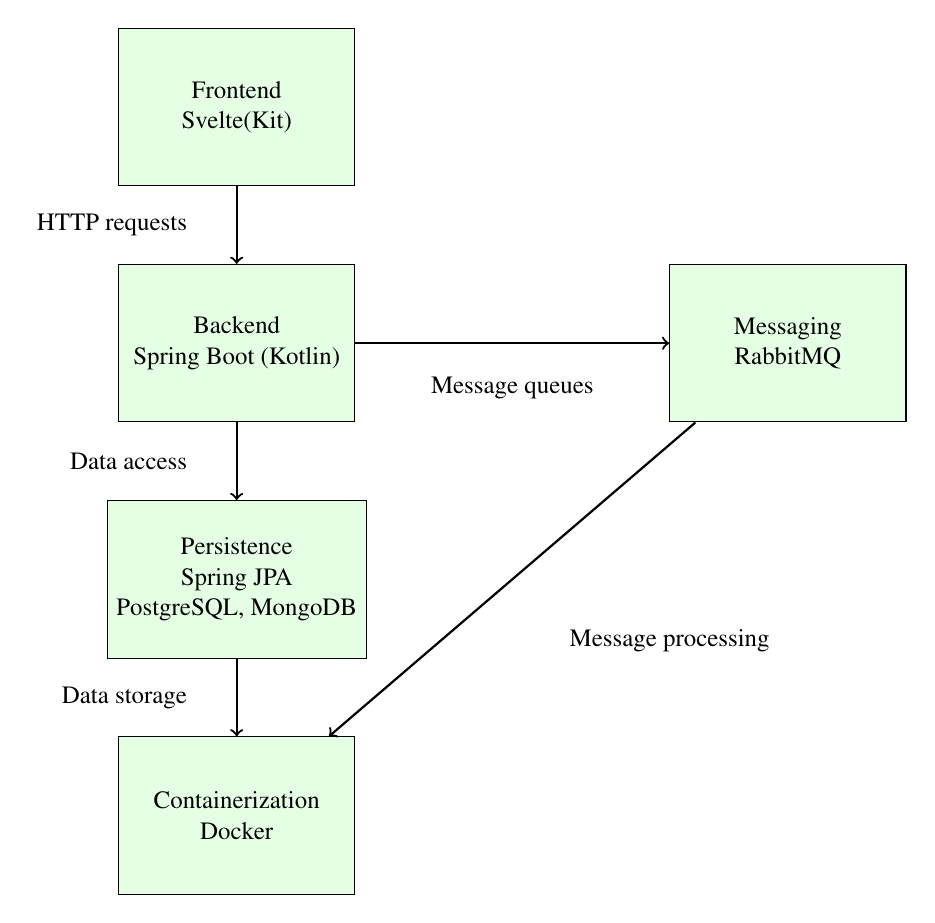
\begin{tikzpicture}[node distance=3cm, auto, font=\small]
    % Define the blocks for each component
    \node (frontend) [draw, rectangle, fill=green!10, text centered, minimum height=2cm, minimum width=3cm, align=center] {Frontend \\ Svelte(Kit)};
    \node (backend) [draw, rectangle, fill=green!10, below of=frontend, text centered, minimum height=2cm, minimum width=3cm, align=center] {Backend \\ Spring Boot (Kotlin)};
    \node (persistence) [draw, rectangle, fill=green!10, below of=backend, text centered, minimum height=2cm, minimum width=3cm, align=center] {Persistence \\ Spring JPA \\ PostgreSQL, MongoDB};
    \node (messaging) [draw, rectangle, fill=green!10, right of=backend, xshift=4cm, text centered, minimum height=2cm, minimum width=3cm, align=center] {Messaging \\ RabbitMQ};
    \node (container) [draw, rectangle, fill=green!10, below of=persistence, text centered, minimum height=2cm, minimum width=3cm, align=center] {Containerization \\ Docker};
    % Draw arrows to show the flow of interaction
    \draw[->, thick] (frontend) -- (backend) node[midway, left, xshift=-0.5cm] {HTTP requests};
    \draw[->, thick] (backend) -- (persistence) node[midway, left, xshift=-0.5cm] {Data access};
    \draw[->, thick] (backend) -- (messaging) node[midway, below, yshift=-0.3cm] {Message queues};
    \draw[->, thick] (persistence) -- (container) node[midway, left, xshift=-0.5cm] {Data storage};
    \draw[->, thick] (messaging) -- (container) node[midway, below, yshift=-0.5cm, xshift=2cm] {Message processing};
\end{tikzpicture}

\caption{Architecture of FeedApp}
\label{fig:architecture}
\end{figure}

\subsection{Backend}
We will now look into how the Kotlin code is organized. We use Kotlin with Spring Boot as the backend. The code is organized into three main services: EventService, PollService, and UserService. These handle the business logic. We also have class JwtService,  which provides token management for authentication.
 
\vspace{2cm}
\begin{figure}[H]
\centering
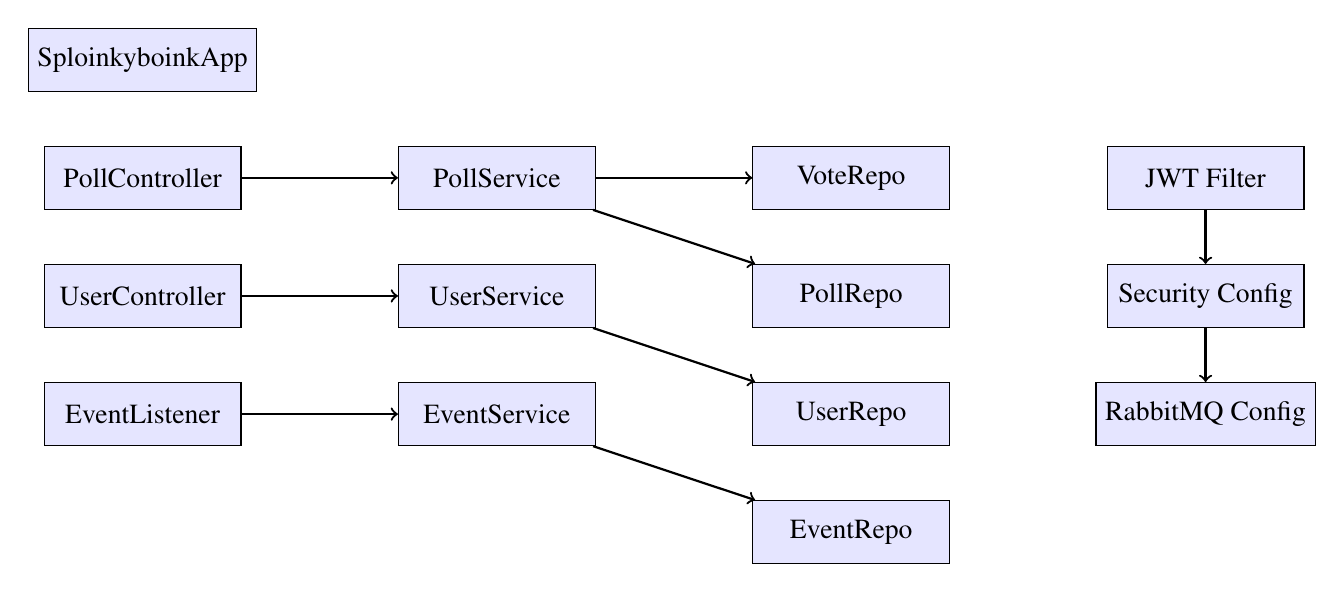
\begin{tikzpicture}[node distance=1.5cm]
% Define UML class styles
\tikzstyle{class} = [rectangle, draw=black, fill=blue!10, text centered, minimum height=0.8cm, minimum width=2.5cm]
\tikzstyle{arrow} = [->, thick, draw=black]
% Define nodes (classes)
\node[class] (SploinkyboinkApplication) {SploinkyboinkApp};
\node[class, below of=SploinkyboinkApplication] (PollController) {PollController};
\node[class, below of=PollController] (UserController) {UserController};
\node[class, below of=UserController] (EventListener) {EventListener};
% Define second layer nodes (Services)
\node[class, right of=PollController, xshift=3cm] (PollService) {PollService};
\node[class, below of=PollService] (UserService) {UserService};
\node[class, below of=UserService] (EventService) {EventService};
% Define third layer nodes (Repositories)
\node[class, right of=PollService, xshift=3cm] (VoteRepository) {VoteRepo};
\node[class, below of=VoteRepository] (PollRepository) {PollRepo};
\node[class, below of=PollRepository] (UserRepository) {UserRepo};
\node[class, below of=UserRepository] (EventRepository) {EventRepo};

% Define fourth layer nodes (Security)
\node[class, right of=VoteRepository, xshift=3cm] (JwtAuthFilter) {JWT Filter};
\node[class, below of=JwtAuthFilter] (SecurityConfig) {Security Config};
% Define fifth layer nodes (Configurations)
\node[class, below of=SecurityConfig] (RabbitMQConfig) {RabbitMQ Config};
% Relationships (arrows)
\draw[arrow] (PollController) -- (PollService);
\draw[arrow] (UserController) -- (UserService);
\draw[arrow] (EventListener) -- (EventService);
\draw[arrow] (PollService) -- (PollRepository);
\draw[arrow] (PollService) -- (VoteRepository);
\draw[arrow] (UserService) -- (UserRepository);
\draw[arrow] (EventService) -- (EventRepository);
\draw[arrow] (JwtAuthFilter) -- (SecurityConfig);
\draw[arrow] (SecurityConfig) -- (RabbitMQConfig);
\end{tikzpicture}

\caption{Overview of the architecture in regards to controllers, services, repositories and configurations}
\label{fig:controller_service_repo_config}
\end{figure}
\vspace{1cm}

\noindent \textbf{Main Application Class}
\begin{itemize}
    \item \textbf{SploinkyboinkApp}: The central class responsible for initializing and running the application.
\end{itemize}

\noindent \textbf{Controllers}
\begin{itemize}
    \item \textbf{PollController}: Manages HTTP requests related to polls.
    \item \textbf{UserController}: Handles user-related HTTP requests.
    \item \textbf{VoteController}: Processes vote-related HTTP requests.
    \item \textbf{EventListener}: Handles event-triggered actions.
\end{itemize}

\noindent \textbf{Services (Business Logic)}
\begin{itemize}
    \item \textbf{EventService}: Logs events such as user votes and poll creation/editing.
    \item \textbf{PollService}: Manages polls and voting logic.
    \item \textbf{UserService}: Handles user registration, authentication, and data operations.
    \item \textbf{VoteService}: Manages vote-related logic.
    \item \textbf{JwtService}: Provides JWT token management for authentication.
\end{itemize}

\noindent \textbf{Repositories (Data Access)}
\begin{itemize}
    \item \textbf{PollRepo}: Interacts with the database for poll-related data.
    \item \textbf{UserRepo}: Manages user data persistence.
    \item \textbf{VoteRepo}: Handles database operations for votes.
    \item \textbf{EventRepo}: Supports event-related data storage and access.
\end{itemize}

\noindent \textbf{Security and Messaging}
\begin{itemize}
    \item \textbf{Security Config}: Configures application-wide security settings and authentication mechanisms.
    \item \textbf{JWT Filters}: Ensures secure token-based authentication.
    \item \textbf{RabbitMQ Config}: Sets up RabbitMQ for message processing and event handling.
\end{itemize}

\vspace{0.5cm}
\noindent \textbf{Achieved functionalities}
\begin{itemize}
    \item \textbf{Polling Functionality}: Users can create, manage, and participate in polls, with their votes accurately captured and stored.
    \item \textbf{Event Tracking}: Tracks important user actions, enabling auditing or analytics.
    \item \textbf{User Management}: Ensures secure user authentication and management through validation mechanisms.
    \item \textbf{Integration with Messaging}: RabbitMQ integration supports a scalable, event-driven architecture, enabling the decoupling of services and enhancing overall application performance.
\end{itemize}

\section{Technology Assessment}
\label{sec:technology}



Introduce in (sufficient) depth the key concepts and architecture of the chosen software technology. As part if this, you may consider using a running example to introduce the technology.

This part and other parts of the report probably needs to refer to
figures. Figure~\ref{fig:framework} from \cite{brown:96} just
illustrates how figure can be included in the report.

\begin{figure}[thb]
	\centering
	\includegraphics[scale=0.5]{figs/framework.png}
	\caption{Software technology evaluation framework.}
	\label{fig:framework}
\end{figure}

\subsection{Descriptive Modeling}

write where the technology comes from, its history, its context and what problem it solves.
Consider drawing a graph like in \cite{brown:96}.


Kotlin, developed by JetBrains (the Czech software company behind IntelliJ IDEA), is named after Kotlin Island in the Gulf of Finland, near St. Petersburg. JetBrains introduced Kotlin in 2011 as a modern language addressing limitations encountered with Java. The first stable release (Kotlin 1.0) arrived in 2016 and gained traction among Android developers quickly. In 2017, Google endorsed Kotlin as an official language for Android development, a significant boost in adoption. In 2020, JetBrains and Google launched the Kotlin Foundation, solidifying its role in JVM and Android development. Kotlin’s ongoing development focuses on multi-platform capabilities, broadening its use beyond JVM and Android to include web, iOS, and server applications. Kotlin is a statically typed language that compiles to Java bytecode, running on the Java Virtual Machine (JVM), which allows compatibility with Java libraries and frameworks. Designed for safety, conciseness, and interoperability with Java, Kotlin is particularly valuable in three contexts:

\begin{itemize}
    \item \textbf{Android Development}: Kotlin’s concise syntax and enhanced safety features make it a preferred choice in Android development.
    \item \textbf{Server-Side Development}: Kotlin’s seamless integration with JVM-based frameworks like Spring Boot facilitates its use in server applications.
    \item \textbf{Multi-Platform Development}: Kotlin Multiplatform and Kotlin/Native enable shared codebases across platforms, including mobile, web, and desktop applications.
\end{itemize}



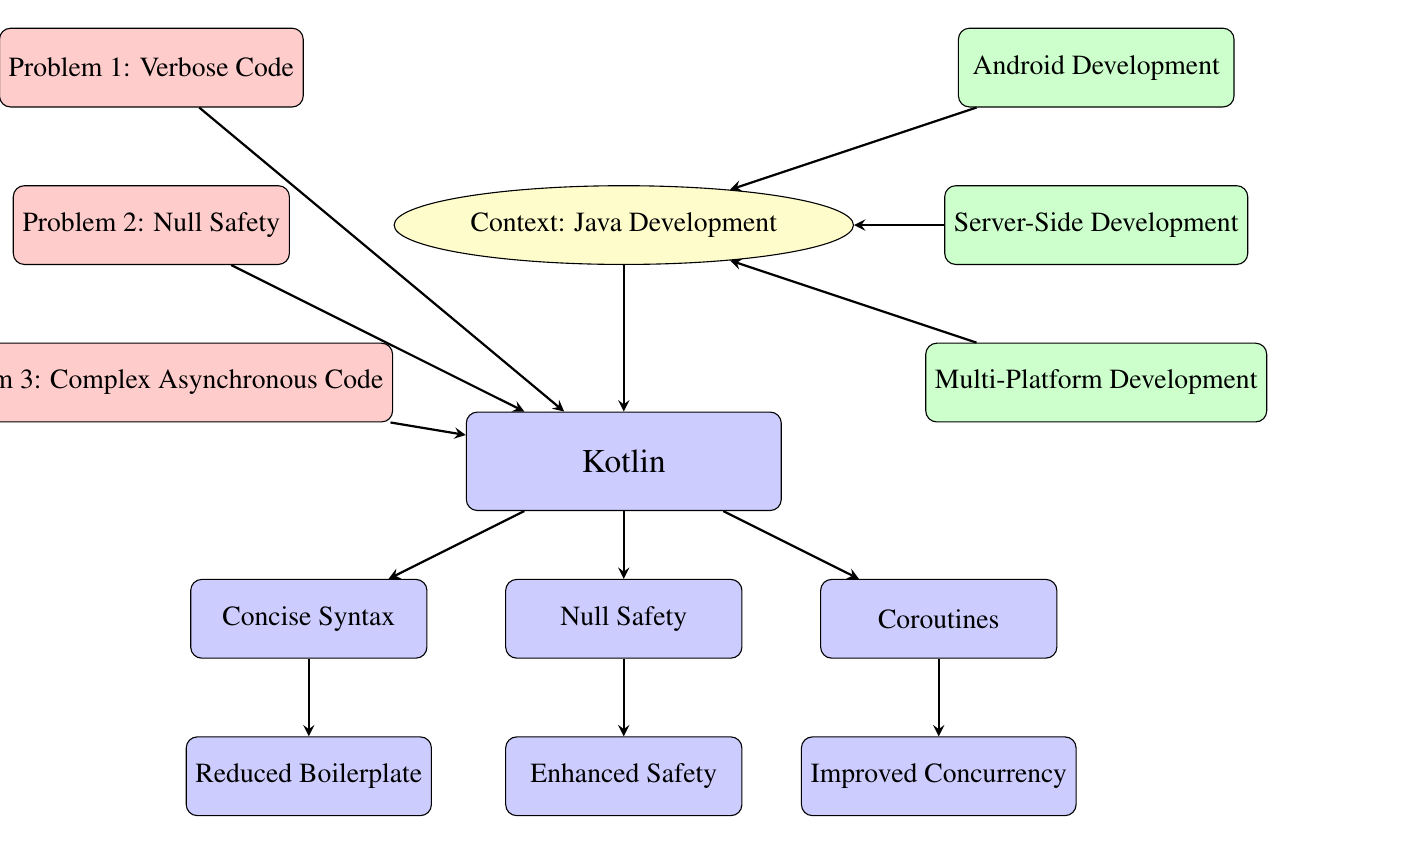
\begin{tikzpicture}[node distance=2cm]

\hspace*{-1.5cm}  % Shifts everything 1.5 cm to the left

% Define block styles
\tikzstyle{block} = [rectangle, rounded corners, minimum width=3cm, minimum height=1cm, text centered, draw=black, fill=blue!20]
\tikzstyle{problem} = [rectangle, rounded corners, minimum width=3cm, minimum height=1cm, text centered, draw=black, fill=red!20]
\tikzstyle{context} = [ellipse, minimum width=4cm, minimum height=1cm, text centered, draw=black, fill=yellow!20]
\tikzstyle{arrow} = [thick,->,>=stealth]
\tikzstyle{usecase} = [rectangle, rounded corners, minimum width=3.5cm, minimum height=1cm, text centered, draw=black, fill=green!20]

% Nodes
\node (problem1) [problem] {Problem 1: Verbose Code};
\node (problem2) [problem, below of=problem1] {Problem 2: Null Safety};
\node (problem3) [problem, below of=problem2] {Problem 3: Complex Asynchronous Code};
\node (context) [context, right of=problem2, xshift=4cm] {Context: Java Development};
\node (kotlin) [block, below of=context, yshift=-1cm, minimum width=4cm, minimum height=1.25cm, font=\large] {Kotlin};

% Spread out the blue boxes
\node (feature1) [block, below of=kotlin, xshift=-4cm] {Concise Syntax};
\node (feature2) [block, below of=kotlin] {Null Safety};
\node (feature3) [block, below of=kotlin, xshift=4cm] {Coroutines};

% Spread out the benefits
\node (benefit1) [block, below of=feature1] {Reduced Boilerplate};
\node (benefit2) [block, below of=feature2] {Enhanced Safety};
\node (benefit3) [block, below of=feature3] {Improved Concurrency};

% Use cases (stacked vertically)
\node (usecase1) [usecase, above of=context, xshift=6cm] {Android Development};
\node (usecase2) [usecase, below of=usecase1] {Server-Side Development};
\node (usecase3) [usecase, below of=usecase2] {Multi-Platform Development};

% Arrows
\draw [arrow] (problem1) -- (kotlin);
\draw [arrow] (problem2) -- (kotlin);
\draw [arrow] (problem3) -- (kotlin);
\draw [arrow] (context) -- (kotlin);
\draw [arrow] (kotlin) -- (feature1);
\draw [arrow] (feature1) -- (benefit1);
\draw [arrow] (kotlin) -- (feature2);
\draw [arrow] (feature2) -- (benefit2);
\draw [arrow] (kotlin) -- (feature3);
\draw [arrow] (feature3) -- (benefit3);

% Arrows from use cases to context (yellow oval)
\draw [arrow] (usecase1) -- (context);
\draw [arrow] (usecase2) -- (context);
\draw [arrow] (usecase3) -- (context);

\end{tikzpicture}

\vspace{1cm}

Kotlin is addressing some of Java's limitations. Kotlin as a programming language has many strengths:
\\
\textbf{Conciseness and Readability}: Kotlin’s streamlined syntax reduces repetitive code, improving readability and maintainability. This conciseness also minimizes potential sources of error and makes the codebase easier to work with.

\textbf{Null Safety}: Kotlin’s type system helps prevent NullPointerExceptions by distinguishing between nullable and non-nullable types. This feature significantly reduces bugs related to null handling, a frequent issue in Java.
\textbf{Asynchronous Programming with Coroutines}: Kotlin’s coroutines offer a simplified approach to asynchronous programming, enabling more efficient, non-blocking code execution ideal for network requests or tasks involving resource waits.

\textbf{Interoperability with Java}: Kotlin’s full compatibility with Java allows teams to gradually integrate Kotlin into existing Java applications. This flexibility is advantageous for modernization efforts without requiring a complete code rewrite.

\textbf{Multi-Platform Support}: Kotlin’s multiplatform capabilities allow for shared business logic across platforms, reducing code duplication and streamlining development for applications targeting Android, iOS, web, and server environments.

\textbf{Functional Programming Features}: Kotlin includes extension functions, higher-order functions, and lambdas, allowing more expressive, modular code. These features support functional programming, further enhancing code flexibility and promoting cleaner architecture.

\textbf{Data Classes}: Kotlin’s data classes simplify the creation of classes primarily used for holding data by automatically generating common methods like \texttt{equals()}, \texttt{hashCode()}, and \texttt{toString()}, streamlining data handling.


\subsection{Experiment Design}

Write you hypotheses about what benefits the technology bring and how you can support or reject them via experiments.

\maketitle

\section*{Improved Development Speed and Code Conciseness}

\textbf{Hypothesis:} Using Kotlin will reduce development time due to its concise syntax. This is expected to simplify tasks such as user, poll, and vote management.

\textbf{Experiment:} Compare the implementation time for key functionalities (e.g., user creation, poll management, and vote handling) between Kotlin and Java. Measure the lines of code required to implement the same logic in both languages and track developer productivity through task completion rates.

\section*{Enhanced Safety with Null Safety}

\textbf{Hypothesis:} Kotlin’s null safety features will reduce runtime exceptions related to null pointer errors, especially in scenarios where entities (like User, Poll, or Vote) might not exist, which would otherwise cause crashes in Java.

\textbf{Experiment:} Introduce null values in critical parts of the business logic (e.g., missing users or votes) and measure the number of runtime exceptions in both Kotlin and Java. Monitor the resilience of the application in handling missing data.

\section*{Simplified Asynchronous Voting Process}

\textbf{Hypothesis:} Kotlin coroutines will streamline asynchronous handling of voting logic, improving response time and scalability during high voting activity.

\textbf{Experiment:} Implement the voting logic using Kotlin coroutines, then simulate high volumes of voting requests. Compare the application’s response times and memory usage with a similar Java implementation using standard concurrency methods.

\section*{Cross-Platform Code Sharing Potential}

\textbf{Hypothesis:} Kotlin Multiplatform would enable code sharing for the voting logic between a potential mobile client and backend, reducing duplicated logic and ensuring consistency across platforms.

\textbf{Experiment:} Set up a prototype of a shared code module containing core voting functions for both the backend and an Android client. Measure code duplication and maintenance requirements, assessing potential consistency improvements.


\subsection{Experiment Evaluation}

Write about the results of your experiments, either via personal experience reports, quantitative benchmarks, a demostrator case study or a combination of multiple approaches.


For some reports you may have to include a table with experimental
results are other kinds of tables that for instance compares
technologies. Table~\ref{tab:results} gives an example of how to create a table.

\begin{table}[bth]
	\centering
	\begin{tabular}{llrrrrrr}
		Config & Property & States & Edges & Peak & E-Time & C-Time & T-Time
		\\ \hline \hline
		22-2 & A   &    7,944  &   22,419  &  6.6  \%  &  7 ms & 42.9\% &  485.7\% \\
		22-2 & A   &    7,944  &   22,419  &  6.6  \%  &  7 ms & 42.9\% &  471.4\% \\
		30-2 & B   &   14,672  &   41,611  &  4.9  \%  & 14 ms & 42.9\% &  464.3\% \\
		30-2 & C   &   14,672  &   41,611  &  4.9  \%  & 15 ms & 40.0\% &  420.0\% \\ \hline
		10-3 & D   &   24,052  &   98,671  & 19.8  \%  & 35 ms & 31.4\% &  285.7\% \\
		10-3 & E   &   24,052  &   98,671  & 19.8  \%  & 35 ms & 34.3\% &  308.6\% \\
		\hline \hline
	\end{tabular}
	\caption{Selected experimental results on the communication protocol example.}
	\label{tab:results}
\end{table}


\section*{1. Concise Syntax}

\textbf{Hypothesis}: Kotlin's syntax will be more concise and less error-prone compared to Java’s verbose syntax.

\textbf{Experiment Example}:
\begin{itemize}
    \item \textbf{Kotlin} (Data class):
    \begin{verbatim}
    data class Person(val name: String, val age: Int)
    \end{verbatim}
    
    \item \textbf{Java} (Full class):
    \begin{verbatim}
    public class Person {
        private String name;
        private int age;

        public Person(String name, int age) {
            this.name = name;
            this.age = age;
        }

        public String getName() { return name; }
        public int getAge() { return age; }
        @Override public String toString() { return "Person{name='" + name + "', age=" + age + '}'; }
    }
    \end{verbatim}
\end{itemize}

\textbf{Conclusion}: Kotlin's \texttt{data class} reduces the need for boilerplate code (like getters, setters, and \texttt{toString()}), making the code more concise and error-resistant. Java’s verbose approach introduces potential for mistakes and increases code length.

\section*{2. Null Safety}

\textbf{Hypothesis}: Kotlin’s null safety features will reduce runtime errors due to null dereferencing compared to Java’s manual null checks.

\textbf{Experiment Example}:
\begin{itemize}
    \item \textbf{Kotlin} (Null safety):
    \begin{verbatim}
    fun greet(name: String?) {
        println("Hello, ${name ?: "Guest"}!")
    }
    greet(null)  // Output: Hello, Guest!
    \end{verbatim}
    
    \item \textbf{Java} (Manual null check):
    \begin{verbatim}
    public void greet(String name) {
        if (name == null) {
            name = "Guest";
        }
        System.out.println("Hello, " + name);
    }
    greet(null);  // Output: Hello, Guest!
    \end{verbatim}
\end{itemize}

\textbf{Conclusion}: Kotlin’s \texttt{null} safety ensures that nullability is explicitly handled using \texttt{?} and \texttt{?:}, reducing runtime errors. Java’s manual null checks are error-prone and can be easily missed, leading to potential \texttt{NullPointerException} risks.

\section*{3. Coroutines (Asynchronous Programming)}

\textbf{Hypothesis}: Kotlin’s coroutines will provide a more efficient and readable way to handle asynchronous tasks than Java’s traditional threading model.

\textbf{Experiment Example}:
\begin{itemize}
    \item \textbf{Kotlin} (Coroutines):
    \begin{verbatim}
    import kotlinx.coroutines.*

    suspend fun fetchData() {
        delay(1000)
        println("Data fetched")
    }

    fun main() = runBlocking {
        launch { fetchData() }
    }
    \end{verbatim}
    
    \item \textbf{Java} (Threads):
    \begin{verbatim}
    public class Main {
        public static void fetchData() {
            try {
                Thread.sleep(1000);
                System.out.println("Data fetched");
            } catch (InterruptedException e) {
                e.printStackTrace();
            }
        }

        public static void main(String[] args) {
            Thread thread = new Thread(() -> fetchData());
            thread.start();
        }
    }
    \end{verbatim}
\end{itemize}

\textbf{Conclusion}: Kotlin coroutines simplify asynchronous code, making it more readable and reducing boilerplate. Java’s thread-based approach requires more code and is harder to manage due to explicit thread handling and synchronization.




\section{Prototype Implementation}
\label{sec:implementation}

This section should provide brief details of how the prototype has been implemented.
You may want to use come code snippets here, but only focus on core features and aspects.
You are not meant to copy/paste your whole application code into the report.
Focus for instance how other developers may run your application and how they might develop it further...


The example below shows how you may include code. There are similar
styles for many other langages - in case you do not use Java in your
project. You can wrap the listing into a figure in case you need to
refer to it. How to create a figure was shown in Section~\ref{sec:technology}.

\lstinputlisting[language=java]{code/BoksVolum.java}


\subsection{Backend}

We will now look into how the Kotlin code is organized. We use Kotlin with Spring Boot as the backend. The code is organized into three main services: EventService, PollService, and UserService. Here’s a high-level overview of what each service does:
\begin{itemize}
    \item \textbf{EventService:}
    \begin{itemize}
        \item \textbf{Logging Events:} This service is responsible for logging various events related to polls and votes. It saves events to a database and sends messages to a RabbitMQ queue.
        \item \textbf{Event Types:} It handles specific types of events such as:
        \begin{itemize}	
            \item \textbf{VoteEvent:} When a user votes on a poll.
            \item \textbf{PollCreated:} When a new poll is created.
            \item \textbf{PollEdited:} When an existing poll is edited.
        \end{itemize}
        The events include details such as the poll ID, the question, options, and timestamp.
    \end{itemize}

    \item \textbf{PollService:}
    \begin{itemize}
        \item \textbf{Poll Management:} This service manages the lifecycle of polls, including creating, retrieving, editing, and deleting polls.
        \item \textbf{Voting Logic:} It also manages voting on polls, ensuring that users can only vote once, that polls are active, and allowing users to edit or delete their votes.
        \item \textbf{Results Calculation:} It calculates and retrieves the results of the polls based on the votes received.
    \end{itemize}

    \item \textbf{UserService:}
    \begin{itemize}
        \item \textbf{User Management:} This service handles user registration, authentication, and management. It ensures that users' usernames and emails are unique and validates passwords against defined criteria.
        \item \textbf{CRUD Operations:} It provides functionality to create, read, update, and delete user information.
    \end{itemize}

    \item \textbf{Achievements of the Code:}
    \begin{itemize}
        \item \textbf{Polling Functionality:} The application allows users to create, manage, and participate in polls, capturing user votes and managing their options.
        \item \textbf{Event Tracking:} It tracks important actions within the application, such as when polls are created or edited, and when votes are cast, providing a basis for auditing or analytics.
        \item \textbf{User Management:} It provides security by validation of users.
        \item \textbf{Integration with Messaging:} By integrating RabbitMQ, it supports event-driven architecture, allowing for scalability and decoupling of services.
    \end{itemize}
\end{itemize}





\section{Conclusions}
\label{sec:conclusion}

Reflecting on our development experience, Kotlin has proven to be a valuable asset in simplifying backend development, particularly when working with Spring and JPA. Its concise syntax and strong type safety have contributed to a cleaner, more maintainable codebase, reducing the potential for errors while improving productivity.
Kotlin’s seamless interoperability with Java has allowed us to integrate it with the frameworks without friction, leveraging established Java libraries alongside Kotlin's modern features.

Throughout the development process, Kotlin’s compatibility with Spring and JPA frameworks has been especially beneficial.
It has enabled us to take full advantage of the expressive nature of Kotlin while adhering to the conventions and strengths of these frameworks.
The language’s null safety and ability to streamline repetitive code have further contributed to smoother workflows and faster development.

The overall experience with Kotlin has been positive, enhancing both the efficiency and clarity of backend development.
Its alignment with developer needs, combined with its growing ecosystem and community support, might ensure a continued relevance in modern software engineering.

In conclusion, Kotlin’s adoption has not only streamlined our backend development processes but has also provided a development experience that is intuitive and enjoyable.
By combining the reliability of Java, its libraries and frameworks with the innovations of a modern programming language, Kotlin has positioned itself as an essential part of our development toolkit, enabling us to deliver robust and maintainable solutions effectively.


\bibliographystyle{plain}
\bibliography{report.bib}

\end{document}
